% =====================================================================
% SOEN 6011 -- Deliverable 2 -- Presentation slides
% Konan Brandon -- 40373534
%
% Compile:  pdflatex slides.tex
% Matches the Beamer/Madrid style used in Deliverable 1.
% =====================================================================

\documentclass{beamer}
\usetheme{Madrid}

\usepackage[utf8]{inputenc}
\usepackage[T1]{fontenc}
\usepackage{graphicx}
\usepackage{amsmath}
\usepackage{booktabs}
\usepackage{hyperref}
\usepackage{listings}
\usepackage{xcolor}

\graphicspath{{../screenshots/}{screenshots/}{./}}

\lstset{
  basicstyle=\ttfamily\tiny,
  breaklines=true,
  frame=single,
  showstringspaces=false
}

\title{F2: tan(x)}
\subtitle{SOEN 6011 --- Deliverable 2}
\author{Konan Brandon}
\institute{Student ID: 40373534\\[0.3cm]
\small\url{https://github.com/Brand0-code/soen6011-tan-calculator}}
\date{Summer 2026}

\begin{document}

\frame{\titlepage}

\begin{frame}{Agenda}
  \tableofcontents
\end{frame}

% =====================================================================
\section{Problem 5: Implementation from Scratch}

\begin{frame}{What ``from scratch'' meant}
  \begin{itemize}
    \item No \texttt{math} module. $\pi$ is a literal constant.
    \item No factorial, no built-in trigonometry.
    \item Permitted: conversion, arithmetic, output, interface.
  \end{itemize}
  \vfill
  Six subordinate functions had to be written:
  \begin{center}
  \small
  \texttt{validate\_number} \quad \texttt{degrees\_to\_radians} \quad
  \texttt{\_nearest\_integer}\\
  \texttt{reduce\_range} \quad \texttt{sine} / \texttt{cosine} \quad
  \texttt{compute\_tan}
  \end{center}
\end{frame}

\begin{frame}{Series without factorials}
  \[
    \sin(x) = x - \frac{x^{3}}{3!} + \frac{x^{5}}{5!} - \cdots
  \]
  Dividing one term by the previous:
  \[
    \frac{x^{5}/5!}{x^{3}/3!} = \frac{x^{2}}{4\cdot 5}
    \quad\Longrightarrow\quad
    t_{k+1} = t_{k}\cdot\frac{-x^{2}}{(2k)(2k+1)}
  \]
  \begin{itemize}
    \item One multiply and one divide per term.
    \item No factorial, no power, nothing overflows.
    \item Stops when $|t_k| < 10^{-15}$ --- not at a fixed count.
  \end{itemize}
\end{frame}

\begin{frame}{Range reduction: why $\pi$, not $2\pi$}
  \begin{itemize}
    \item $\sin$ and $\cos$ both change sign over $\pi$ ---
          the signs cancel in the ratio.
    \item So $\tan(x + \pi) = \tan(x)$: the period is $\pi$.
    \item Reducing by $\pi$ lands the argument in
          $[-\pi/2,\ \pi/2]$, where the series converges fastest.
    \item It also collapses \emph{every} asymptote onto one check.
  \end{itemize}
  \vfill
  \begin{center}
    Without this, $x = 1000$ would be unusable.
  \end{center}
\end{frame}

\begin{frame}{Error handling}
  \begin{center}
  \texttt{TanCalculatorError}\\
  \vspace{0.2cm}
  $\swarrow$ \hspace{2.2cm} $\searrow$\\
  \vspace{0.2cm}
  \texttt{UndefinedTangentError} \hspace{0.5cm}
  \texttt{InvalidInputError}
  \end{center}
  \vfill
  \begin{itemize}
    \item One base class, so the interface catches both with a single
          handler.
    \item Messages say what to enter instead --- never a stack trace.
  \end{itemize}
\end{frame}

\begin{frame}{The graphical interface}
  \begin{columns}
    \column{0.5\textwidth}
      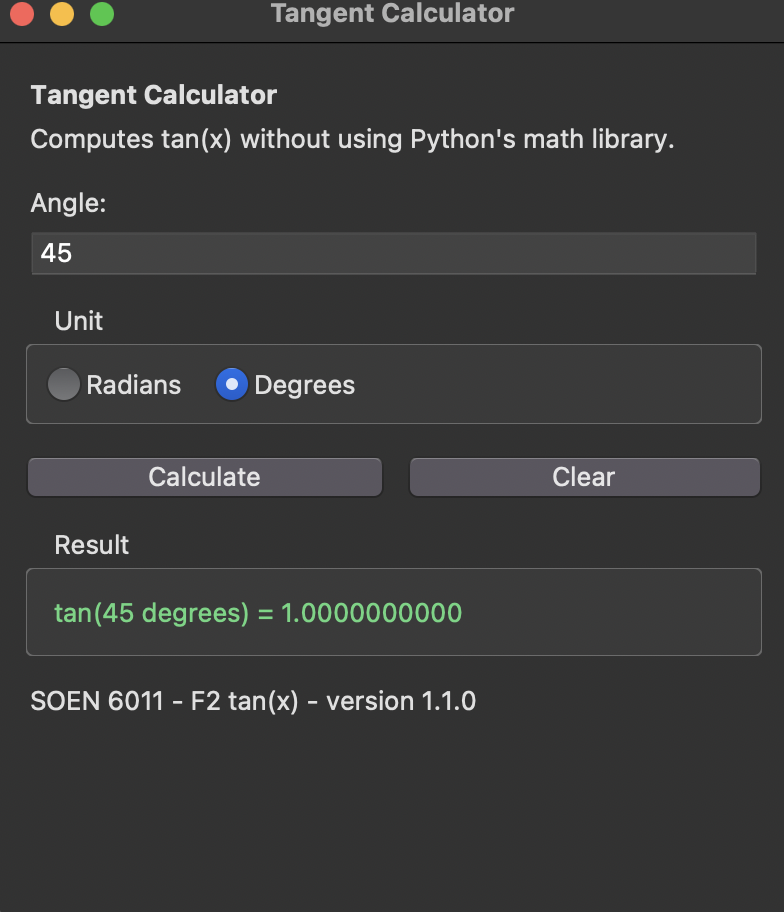
\includegraphics[width=\textwidth]{gui_01_success.png}
    \column{0.5\textwidth}
      \small
      \begin{itemize}
        \item Tkinter; no arithmetic in this module
        \item Radians or degrees
        \item Return calculates, Escape clears
        \item Labels on every control
        \item Outcome stated in words, not colour alone
      \end{itemize}
  \end{columns}
\end{frame}

\begin{frame}{Errors the user can act on}
  \begin{columns}
    \column{0.33\textwidth}
      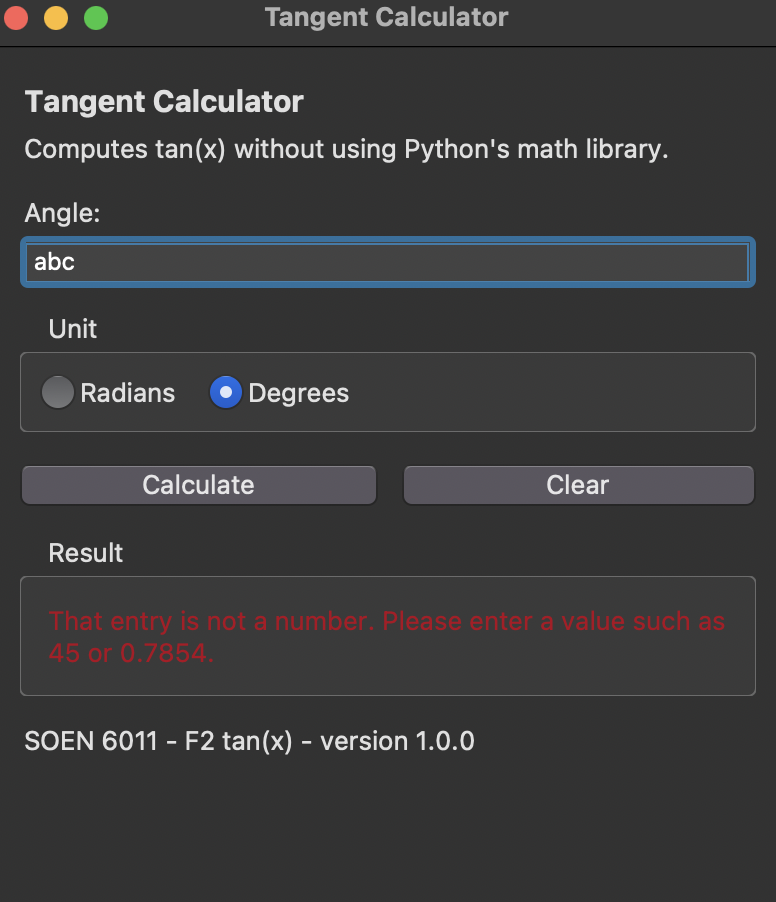
\includegraphics[width=\textwidth]{gui_02_asymptote_error.png}
    \column{0.33\textwidth}
      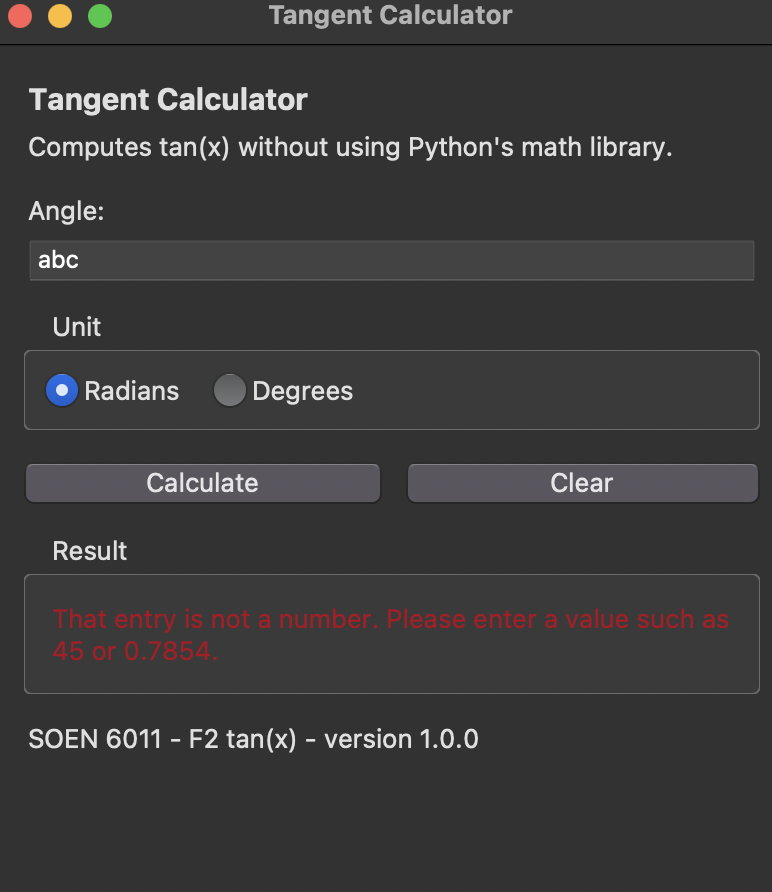
\includegraphics[width=\textwidth]{gui_03_invalid_input.png}
    \column{0.33\textwidth}
      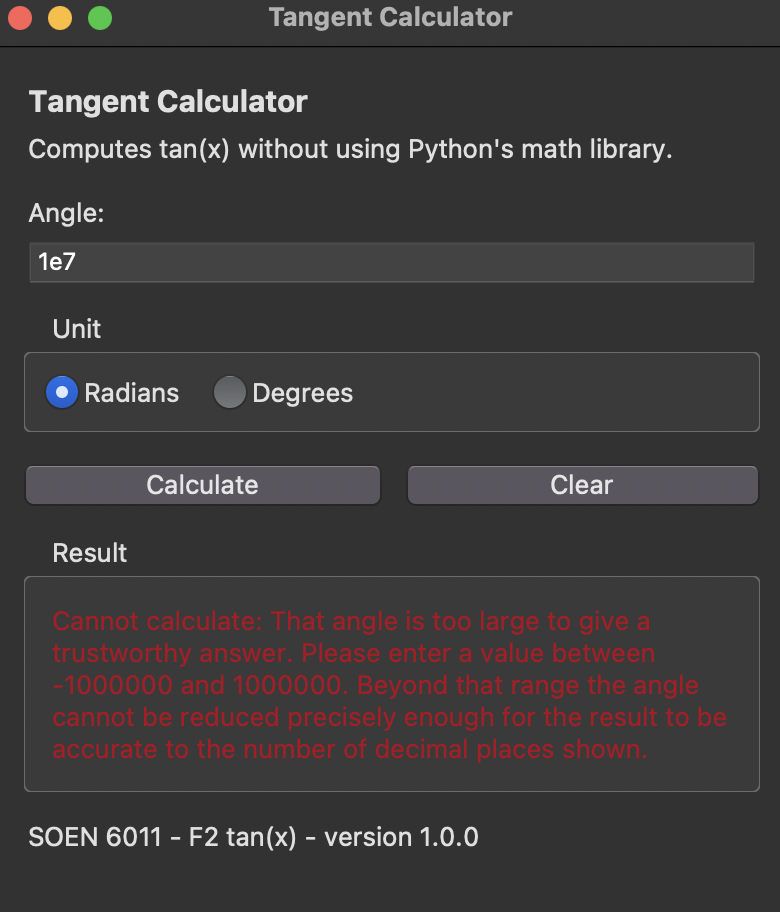
\includegraphics[width=\textwidth]{gui_04_magnitude_guard.png}
  \end{columns}
  \vfill
  \centering
  \small Asymptote \hspace{1.6cm} Non-numeric \hspace{1.2cm}
  Out of range
\end{frame}

\begin{frame}{Verification: 44 of 44 checks}
  \centering
  \small
  \begin{tabular}{lrr}
    \toprule
    \textbf{Angle (rad)} & \textbf{This program} &
    \textbf{Rel. diff.} \\
    \midrule
    $\pi/4$   & 1.0000000000    & $1.1\times10^{-16}$ \\
    2.0       & $-2.1850398633$ & $2.0\times10^{-16}$ \\
    1000.0    & 1.4703241557    & $3.8\times10^{-14}$ \\
    1.57      & 1255.7655915007 & $3.5\times10^{-14}$ \\
    $10^{6}$  & $-0.3736244539$ & $9.4\times10^{-11}$ \\
    \bottomrule
  \end{tabular}
  \vfill
  \footnotesize
  Reference: \texttt{math.tan}, imported only in the test harness ---
  never in the implementation.
\end{frame}

\begin{frame}{A defect that reading the code would not reveal}
  \begin{block}{$\tan(10^{15})$}
    Returned $-1.557$. True value $-1.672$.\\
    Wrong in the first decimal --- and \textbf{no error raised}.
  \end{block}
  \vfill
  \centering
  \small
  \begin{tabular}{lrr}
    \toprule
    \textbf{Magnitude} & \textbf{Typical digits} & \textbf{Worst} \\
    \midrule
    $10^{4}$ & 11.7 & 8.8 \\
    $10^{6}$ & 9.7  & 6.8 \\
    $10^{8}$ & 7.7  & 5.1 \\
    \bottomrule
  \end{tabular}
  \vfill
  \footnotesize
  Ten decimal places are displayed. Past $10^{6}$ the worst case
  falls below six correct digits --- so $10^{6}$ is the limit, and
  larger angles are refused with an explanation.
\end{frame}

\begin{frame}{Two faults found by testing, not by reading}
  \begin{enumerate}
    \item \textbf{Silent precision loss} at large arguments.
          Found by comparing against a reference; fixed by a
          documented validated range.
    \item \textbf{Signature mismatch} between the interface and the
          calculation module --- two arguments passed where one was
          defined. Each file was correct alone and wrong together.
  \end{enumerate}
  \vfill
  \begin{center}
    Exhaustive check: all 636{,}620 asymptotes in range
    correctly detected.
  \end{center}
\end{frame}

% =====================================================================
\section{Problem 6: Version Control}

\begin{frame}{Repository}
  \begin{center}
    \small
    \url{https://github.com/Brand0-code/soen6011-tan-calculator}
  \end{center}
  \vfill
  \begin{itemize}
    \item Public; tagged \texttt{v1.0.0} (Semantic Versioning)
    \item Eight commits, made as the work progressed
    \item Imperative mood; the body states \emph{why}
    \item README: usage, verification, accuracy, validated range
    \item \texttt{.gitignore} keeps platform artefacts out
  \end{itemize}
\end{frame}

\begin{frame}[fragile]{Commit messages}
\begin{lstlisting}
Add verification harness comparing output against math.tan

Checks reference angles, degree conversion, range reduction,
behaviour near asymptotes, undefined points, rejected input,
and the boundary of the accepted range. The math import is
confined to this harness and is absent from the implementation.
\end{lstlisting}
\end{frame}

% =====================================================================
\section{Problem 7: Updated Requirements}

\begin{frame}{What D1 feedback said, and what changed}
  \begin{block}{D1: REQ-001 \ldots REQ-008}
    One flat sequence mixing ``compute the tangent'' with
    ``six decimal places''.
  \end{block}
  \vfill
  \begin{block}{D2: four categories, each with its own sequence}
    \begin{tabular}{ll}
      \texttt{TAN-FR-\textit{nn}}  & functional (12) \\
      \texttt{TAN-UI-\textit{nn}}  & interface (8) \\
      \texttt{TAN-NFR-\textit{nn}} & quality attributes (6) \\
      \texttt{TAN-CON-\textit{nn}} & constraints (3) \\
    \end{tabular}
  \end{block}
\end{frame}

\begin{frame}{Change log}
  \centering
  \small
  \begin{tabular}{lll}
    \toprule
    \textbf{Status} & \textbf{Count} & \textbf{Example} \\
    \midrule
    Unchanged & 4 & REQ-001 $\rightarrow$ TAN-FR-01 \\
    Modified  & 4 & REQ-004 CLI $\rightarrow$ TAN-UI-01 GUI \\
    Added     & 21 & TAN-FR-11 validated range \\
    Removed   & 0 & REQ-004 superseded, not withdrawn \\
    \bottomrule
  \end{tabular}
  \vfill
  \footnotesize
  REQ-003 was \emph{split}: plain language is a quality attribute
  (TAN-NFR-01); ``no stack trace'' is interface behaviour
  (TAN-UI-07).
\end{frame}

\begin{frame}{Why 8 requirements became 29}
  \begin{center}
    Not padding --- a consequence of Problem 5.
  \end{center}
  \vfill
  \begin{itemize}
    \item D1 could leave series evaluation, range reduction and
          termination unstated, because a library did that work.
    \item Prohibiting the library makes each of those a design
          decision.
    \item Every decision carries its own verifiable requirement.
  \end{itemize}
\end{frame}

% =====================================================================
\section{Demonstration}

\begin{frame}{Live demonstration}
  \begin{enumerate}
    \item $45^{\circ}$ \quad $\rightarrow$ \quad 1.0000000000
    \item 1000 radians \quad $\rightarrow$ \quad range reduction works
    \item $90^{\circ}$ \quad $\rightarrow$ \quad undefined, explained
    \item \texttt{abc} \quad $\rightarrow$ \quad not a number
    \item \texttt{1e7} \quad $\rightarrow$ \quad beyond validated range
  \end{enumerate}
  \vfill
  \begin{center}
    \texttt{python tan\_gui.py} --- no IDE, no build step
  \end{center}
\end{frame}

\begin{frame}{Summary}
  \begin{itemize}
    \item Tangent computed from first principles; no library
          arithmetic
    \item Tkinter interface, separated from the calculation
    \item 44 of 44 verification checks pass; Flake8 clean;
          Pylint 10.00/10
    \item Validated range set by measurement, not assumption
    \item Public repository, tagged \texttt{v1.0.0}
    \item Requirements restructured to ISO/IEC/IEEE 29148
  \end{itemize}
  \vfill
  \begin{center}
    \small\url{https://github.com/Brand0-code/soen6011-tan-calculator}

    \vspace{0.3cm}
    \normalsize Thank you --- questions?
  \end{center}
\end{frame}

\end{document}
